\section{Auswertung}
\label{sec:Auswertung}
Aufgrund der Menge der Daten sind die Datensätze im Protokoll nicht mit angegeben und es ist aus Gründen der Lesbarkeit jeder Graph mit einer durchgezogenen Linien
und keinen einzelnen Punkten markiert.
Sie können aber auf Anfrage online zugeschickt werden.\\
\\
Die Wärmeleitfähigkeit von vier unterschiedlichen Metallstäben wird einmal durch eine statische und
eine dynamische Methode bestimmt.

\subsection{Materialkonstanten}
\label{sec:material}
In \autoref{tab:lit} sind die Literaturwerte der Dichten, spezifischen Wärme und Wärmeleitfähigkeit von Messing, Aluminium, Edelstahl und Wasser angegeben.
\begin{table}
  \centering
  \caption{Literaturwerte für Messing, Aluminium und Edelstahl.}
  \label{tab:lit}
  \begin{tabular}{c c c c}
    1 & 1 & 1 & 1 \\
  \end{tabular}
\end{table} 

\subsection{Statische Methode}
\label{sec:stat}

In \autoref{fig:T1T4} sind die zeitlichen Verläufe von $T_1$, $T_4$, $T_5$ und $T_8$ aufgetragen. Diese stellen die vom Peltierelement weiter
entfernten Thermoelemente dar.

\begin{figure}[h]
  \centering
  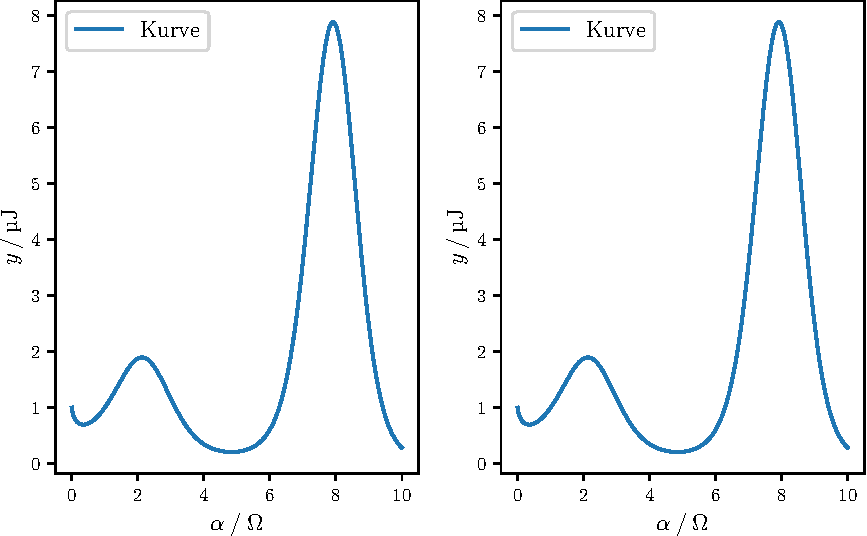
\includegraphics{plot.pdf}
  \caption{Temperaturverlauf der Stäbe außen.}
  \label{fig:T1T4}
\end{figure}
Die Verläufe haben alle eine kurzen Startbereich bis ca. $10 \,\si{\second}$ bei dem die Verläufe nicht
ansteigen. Danach stellt sich bei allen Verläufen eine Sättigungskurve ein.
Dabei fällt auf, dass der Temperaturverlauf des Edelstahlstabs am langsamsten
ansteigt und auch insgesamt die Form der Sättigungskurve abflacht. Weiterhin hat der Edelstahlstab einen längere Startbereich bis ca. $50\,\si{\second}$
bei dem keine Temperaturänderung fest zu stellen ist.\\
\\
Nach $700\,\si{\second}$ hat der Aluminiumstab die höchste Temperatur erreicht. Darauf folgen in absteigender Reihenfolge der breite Messingstab, der schmale Messingstab
und der Edelstahlstab. Demnach hat Aluminium die größe Wärmeleitfähigkeit von den vier Stäben.
\begin{table}[h]
  \centering
  \caption{Äußere Temperatur nach $700\,\si{\second}$.}
  \label{tab:700s}
  \begin{tabular}{c c c c c}
    \toprule
    $t$ & Messing (breit) & Messing (schmal) & Aluminium & Edelstahl \\
    \midrule
    $700\,\si{\second}$ & $47,62\,\si{\celsius}$ & $43,97\,\si{\celsius}$ & $49,15\,\si{\celsius}$ & $35,20\,\si{\celsius}$ \\
    \bottomrule
  \end{tabular}
\end{table}

\subsubsection{Wärmestrom}
\label{sec:waermestrom}
Nun wird der Wärmestrom für jeweils 5 Messwerte bestimmt. Dabei ist $\kappa$ der Literaturwert der Wärmeleitfähigkeit des jeweiligen
Materials, $A$ die Querschnittsfläche und $\frac{\partial T}{\partial x}$ der Temperaturgradient, der als $\frac{\symup{\Delta} T}{\symup{\Delta} x}$
mit $\symup{\Delta}x \approx 3,00\,\si{\centi\meter}$ geschrieben wird.

Die verwendeten fünf Messungen für die Temperaturdifferenzen der jeweiligen Stäbe sind in \autoref{tab:5messungen} angegeben.
\begin{table}[h]
  \centering
  \caption{Temperaturdifferenzen für fünf Messzeiten.}
  \label{tab:5messungen}
  \begin{tabular}{c c c c c}
    \toprule
    $t\,\mathbin{/}\,\si{\second}$ & Messing (breit) & Messing (schmal) & Aluminium & Edelstahl \\
    \midrule
     30\,\si{\second} & 5,68\,\si{\celsius} & 7,07\,\si{\celsius} & 5,69\,\si{\celsius} & 2,33\,\si{\celsius} \\
     60\,\si{\second} & 6,97\,\si{\celsius} & 8,43\,\si{\celsius} & 5,16\,\si{\celsius} & 8,65\,\si{\celsius} \\
    120\,\si{\second} & 5,27\,\si{\celsius} & 6,39\,\si{\celsius} & 3,27\,\si{\celsius} & 12,01\,\si{\celsius} \\
    240\,\si{\second} & 3,22\,\si{\celsius} & 4,44\,\si{\celsius} & 1,91\,\si{\celsius} & 11,44\,\si{\celsius} \\
    480\,\si{\second} & 2,28\,\si{\celsius} & 3,72\,\si{\celsius} & 1,52\,\si{\celsius} & 10,25\,\si{\celsius} \\
    \bottomrule
  \end{tabular}
\end{table}

Die Querschnittsflächen sind für die breiten Messing-, Aluminium- und Edelstahlstäbe durch
\begin{align*}
  A_{\symup{breit}} &= 1,2\,\si{\centi\meter}\cdot 0,4\,\si{\centi\meter} \\
                    &= 0,48\,\si{\centi\meter^2}
\end{align*}
gegeben \cite{sample}. Die Querschnittsfläche des schmalen Messingstabs ist durch
\begin{align*}
  A_{\symup{schmal}} &= 0,7\,\si{\centi\meter}\cdot 0,4\,\si{\centi\meter} \\
                     &= 0,28\,\si{\centi\meter^2}
\end{align*}
gegeben \cite{sample}.
Der Wärmestrom für die Messwerte wird durch \autoref{eqn:Waermefluss} bestimmt. Die Ergebnisse sind in zu finden.

Anschließend werden die Temperaturdifferenzen des breiten Messingstabs $\symup{\Delta}T_{\symup{Messing}}$ und des Edelstahlstabs $\symup{\Delta}T_{\symup{Messing}}$
verglichen. Die Graphen sind in \autoref{fig:Tempdiff} dargestellt.
\begin{figure}[h]
  \centering
  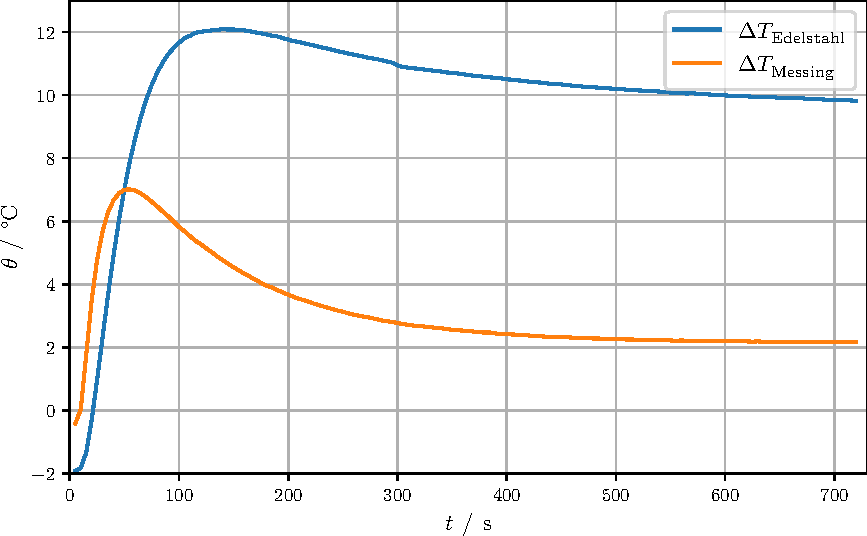
\includegraphics{Tempdiff.pdf}
  \caption{Temperaturdifferenz des breiten Messingstabs und des Edelstahlstabs.}
  \label{fig:Tempdiff}
\end{figure}
Dabei ist fest zu halten, dass die Verläufe bis ca. $50\,\si{\second}$ fast gleich verlaufen.
Durch die bessere Wärmeleitfähigkeit des Messings fällt die Temperaturdifferenz dann aber ab, da die Wärme bis zum äußeren Thermoelement vorgedrungen ist. Danach
stellt sich ab ca. $500\,\si{\second}$ ein Gleichgewicht ein. Für Edelstahl dauert dieser Prozess länger an, da die Wärmeleitfähigkeit geringer ist, so dass sich
das Gleichgewicht erst nach ca. $700\,\si{\second}$ einstellt. Die geringere Wärmeleitfähigkeit des Edelstahls sorgt auch dafür, dass der Verlauf einen höheren Peak
erreicht.

\subsection{Dynamische Methode}
\label{dynam}

\begin{figure}[h]
  \centering
  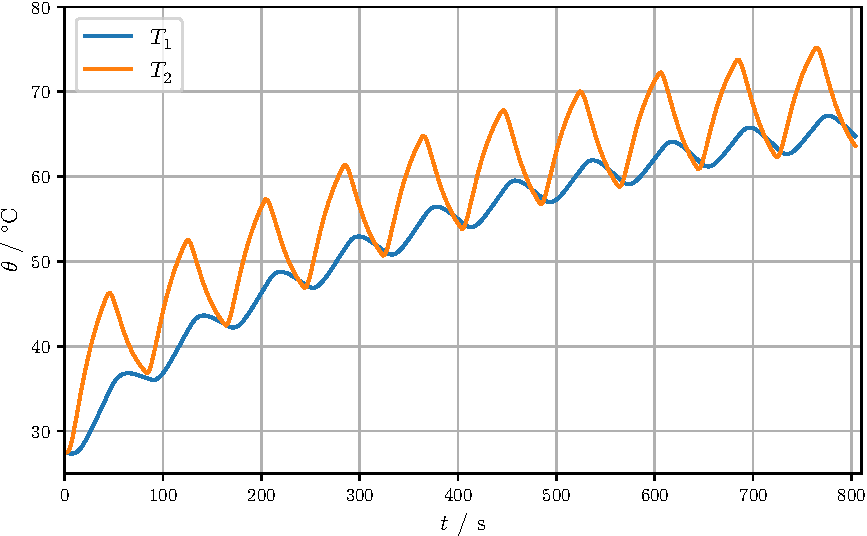
\includegraphics{80sMess.pdf}
  \caption{Temperaturverlauf des breiten Messingstabs.}
  \label{fig:80sMess}
\end{figure}

\begin{figure}[h]
  \centering
  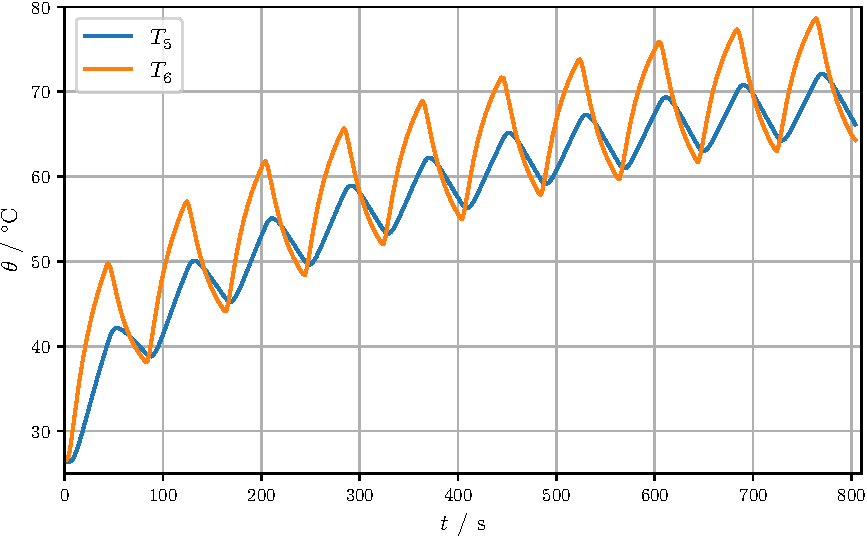
\includegraphics{80sAlu.pdf}
  \caption{Temperaturverlauf des Aluminiumstabs.}
  \label{fig:80sAlu}
\end{figure}

\begin{figure}[h]
  \centering
  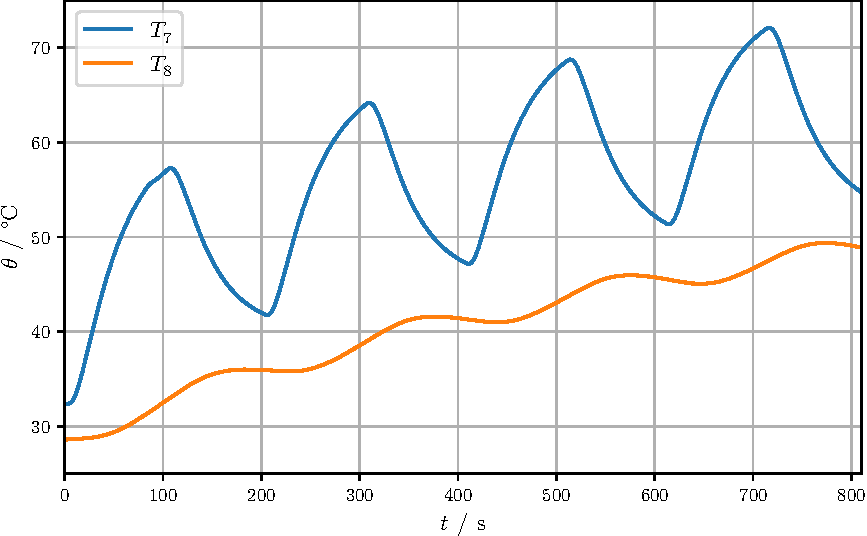
\includegraphics{200sEdelstahl.pdf}
  \caption{Temperaturverlauf des Edelstahlstabs.}
  \label{fig:200sEdelstahl}
\end{figure}
